\documentclass[]{report}
\usepackage{lmodern}
\usepackage{amssymb,amsmath}
\usepackage{ifxetex,ifluatex}
\usepackage{fixltx2e} % provides \textsubscript
\ifnum 0\ifxetex 1\fi\ifluatex 1\fi=0 % if pdftex
  \usepackage[T1]{fontenc}
  \usepackage[utf8]{inputenc}
\else % if luatex or xelatex
  \ifxetex
    \usepackage{mathspec}
  \else
    \usepackage{fontspec}
  \fi
  \defaultfontfeatures{Ligatures=TeX,Scale=MatchLowercase}
\fi
% use upquote if available, for straight quotes in verbatim environments
\IfFileExists{upquote.sty}{\usepackage{upquote}}{}
% use microtype if available
\IfFileExists{microtype.sty}{%
\usepackage{microtype}
\UseMicrotypeSet[protrusion]{basicmath} % disable protrusion for tt fonts
}{}
\usepackage{hyperref}
\hypersetup{unicode=true,
            pdftitle={Homework Part 2},
            pdfauthor={Vinicio Haro; Sang Yoon (Andy) Hwang; Julian McEachern; Jeremy O'Brien; Bethany Poulin},
            pdfborder={0 0 0},
            breaklinks=true}
\urlstyle{same}  % don't use monospace font for urls
\usepackage{color}
\usepackage{fancyvrb}
\newcommand{\VerbBar}{|}
\newcommand{\VERB}{\Verb[commandchars=\\\{\}]}
\DefineVerbatimEnvironment{Highlighting}{Verbatim}{commandchars=\\\{\}}
% Add ',fontsize=\small' for more characters per line
\usepackage{framed}
\definecolor{shadecolor}{RGB}{248,248,248}
\newenvironment{Shaded}{\begin{snugshade}}{\end{snugshade}}
\newcommand{\AlertTok}[1]{\textcolor[rgb]{0.94,0.16,0.16}{#1}}
\newcommand{\AnnotationTok}[1]{\textcolor[rgb]{0.56,0.35,0.01}{\textbf{\textit{#1}}}}
\newcommand{\AttributeTok}[1]{\textcolor[rgb]{0.77,0.63,0.00}{#1}}
\newcommand{\BaseNTok}[1]{\textcolor[rgb]{0.00,0.00,0.81}{#1}}
\newcommand{\BuiltInTok}[1]{#1}
\newcommand{\CharTok}[1]{\textcolor[rgb]{0.31,0.60,0.02}{#1}}
\newcommand{\CommentTok}[1]{\textcolor[rgb]{0.56,0.35,0.01}{\textit{#1}}}
\newcommand{\CommentVarTok}[1]{\textcolor[rgb]{0.56,0.35,0.01}{\textbf{\textit{#1}}}}
\newcommand{\ConstantTok}[1]{\textcolor[rgb]{0.00,0.00,0.00}{#1}}
\newcommand{\ControlFlowTok}[1]{\textcolor[rgb]{0.13,0.29,0.53}{\textbf{#1}}}
\newcommand{\DataTypeTok}[1]{\textcolor[rgb]{0.13,0.29,0.53}{#1}}
\newcommand{\DecValTok}[1]{\textcolor[rgb]{0.00,0.00,0.81}{#1}}
\newcommand{\DocumentationTok}[1]{\textcolor[rgb]{0.56,0.35,0.01}{\textbf{\textit{#1}}}}
\newcommand{\ErrorTok}[1]{\textcolor[rgb]{0.64,0.00,0.00}{\textbf{#1}}}
\newcommand{\ExtensionTok}[1]{#1}
\newcommand{\FloatTok}[1]{\textcolor[rgb]{0.00,0.00,0.81}{#1}}
\newcommand{\FunctionTok}[1]{\textcolor[rgb]{0.00,0.00,0.00}{#1}}
\newcommand{\ImportTok}[1]{#1}
\newcommand{\InformationTok}[1]{\textcolor[rgb]{0.56,0.35,0.01}{\textbf{\textit{#1}}}}
\newcommand{\KeywordTok}[1]{\textcolor[rgb]{0.13,0.29,0.53}{\textbf{#1}}}
\newcommand{\NormalTok}[1]{#1}
\newcommand{\OperatorTok}[1]{\textcolor[rgb]{0.81,0.36,0.00}{\textbf{#1}}}
\newcommand{\OtherTok}[1]{\textcolor[rgb]{0.56,0.35,0.01}{#1}}
\newcommand{\PreprocessorTok}[1]{\textcolor[rgb]{0.56,0.35,0.01}{\textit{#1}}}
\newcommand{\RegionMarkerTok}[1]{#1}
\newcommand{\SpecialCharTok}[1]{\textcolor[rgb]{0.00,0.00,0.00}{#1}}
\newcommand{\SpecialStringTok}[1]{\textcolor[rgb]{0.31,0.60,0.02}{#1}}
\newcommand{\StringTok}[1]{\textcolor[rgb]{0.31,0.60,0.02}{#1}}
\newcommand{\VariableTok}[1]{\textcolor[rgb]{0.00,0.00,0.00}{#1}}
\newcommand{\VerbatimStringTok}[1]{\textcolor[rgb]{0.31,0.60,0.02}{#1}}
\newcommand{\WarningTok}[1]{\textcolor[rgb]{0.56,0.35,0.01}{\textbf{\textit{#1}}}}
\usepackage{graphicx,grffile}
\makeatletter
\def\maxwidth{\ifdim\Gin@nat@width>\linewidth\linewidth\else\Gin@nat@width\fi}
\def\maxheight{\ifdim\Gin@nat@height>\textheight\textheight\else\Gin@nat@height\fi}
\makeatother
% Scale images if necessary, so that they will not overflow the page
% margins by default, and it is still possible to overwrite the defaults
% using explicit options in \includegraphics[width, height, ...]{}
\setkeys{Gin}{width=\maxwidth,height=\maxheight,keepaspectratio}
\IfFileExists{parskip.sty}{%
\usepackage{parskip}
}{% else
\setlength{\parindent}{0pt}
\setlength{\parskip}{6pt plus 2pt minus 1pt}
}
\setlength{\emergencystretch}{3em}  % prevent overfull lines
\providecommand{\tightlist}{%
  \setlength{\itemsep}{0pt}\setlength{\parskip}{0pt}}
\setcounter{secnumdepth}{0}

%%% Use protect on footnotes to avoid problems with footnotes in titles
\let\rmarkdownfootnote\footnote%
\def\footnote{\protect\rmarkdownfootnote}

%%% Change title format to be more compact
\usepackage{titling}

% Create subtitle command for use in maketitle
\providecommand{\subtitle}[1]{
  \posttitle{
    \begin{center}\large#1\end{center}
    }
}

\setlength{\droptitle}{-2em}

  \title{Homework Part 2}
    \pretitle{\vspace{\droptitle}\centering\huge}
  \posttitle{\par}
    \author{Vinicio Haro \\ Sang Yoon (Andy) Hwang \\ Julian McEachern \\ Jeremy O'Brien \\ Bethany Poulin}
    \preauthor{\centering\large\emph}
  \postauthor{\par}
    \date{}
    \predate{}\postdate{}
  
% set plain style for page numbers
\pagestyle{plain}
\raggedbottom

% change font
\usepackage{fontspec}
\setmainfont{Arial}

% create color block quotes
\usepackage[dvipsnames]{xcolor}
\definecolor{navyblue}{RGB}{16, 52, 166}
\definecolor{stealblue}{RGB}{72, 90, 122}
\usepackage{tcolorbox}     
\newtcolorbox{question}[1]{colback=white, colframe=navyblue ,fonttitle=\bfseries, title=#1}

\newtcolorbox{subquestion}[1]{colback=white,colframe=white, coltitle=navyblue!75!black, detach title, before upper={\tcbtitle\quad\hangindent7mm}, title={#1},fonttitle=\bfseries, fontupper=\bfseries}


\usepackage{xcolor}
\usepackage{sectsty}
\usepackage{etoolbox}
\usepackage{titling}

\usepackage{titling}
\pretitle{\begin{flushright}\Huge\color{navyblue}\textbf}
\posttitle{\par\Large\color{gray}Data 624 - Predictive Analytics\linebreak 16 December 2019\end{flushright}}
\preauthor{\begin{flushright}\large \lineskip 0.5em\textbf{Group Members:}\linebreak\textit}
\postauthor{\par\end{flushright}}
\predate{\begin{flushright}\large}
\postdate{\par\end{flushright}}




% remove "chapter" from chapter title
\usepackage{titlesec}
\titleformat{\chapter}
  {\normalfont\color{navyblue}\LARGE\bfseries}{\thechapter}{1em}{}
\titlespacing*{\chapter}{0pt}{3.5ex plus 1ex minus .2ex}{2.3ex plus .2ex}


% margins
\usepackage[margin=1in]{geometry}

% kable 
\usepackage{tabu}
\usepackage{float} 
\usepackage{booktabs}
\usepackage[font={color=navyblue,bf}]{caption}

% multicolumn
\usepackage{multicol}
\usepackage{booktabs}
\usepackage{longtable}
\usepackage{array}
\usepackage{multirow}
\usepackage{wrapfig}
\usepackage{float}
\usepackage{colortbl}
\usepackage{pdflscape}
\usepackage{tabu}
\usepackage{threeparttable}
\usepackage{threeparttablex}
\usepackage[normalem]{ulem}
\usepackage{makecell}
\usepackage{xcolor}

\begin{document}
\maketitle

{
\setcounter{tocdepth}{2}
\tableofcontents
}
\hypertarget{Overview}{%
\chapter*{Getting Started}\label{Overview}}
\addcontentsline{toc}{chapter}{Getting Started}

\hypertarget{overview}{%
\section{Overview}\label{overview}}

Include details on our process in creating this document.

\hypertarget{dependencies}{%
\section{Dependencies}\label{dependencies}}

\begin{Shaded}
\begin{Highlighting}[]
\CommentTok{# Predicitve Modeling}
\KeywordTok{libraries}\NormalTok{(}\StringTok{"AppliedPredictiveModeling"}\NormalTok{, }\StringTok{"mice"}\NormalTok{, }\StringTok{"caret"}\NormalTok{, }\StringTok{"tidyverse"}\NormalTok{, }
    \StringTok{"impute"}\NormalTok{, }\StringTok{"pls"}\NormalTok{, }\StringTok{"caTools"}\NormalTok{, }\StringTok{"mlbench"}\NormalTok{, }\StringTok{"randomForest"}\NormalTok{, }\StringTok{"party"}\NormalTok{, }
    \StringTok{"gbm"}\NormalTok{, }\StringTok{"Cubist"}\NormalTok{, }\StringTok{"rpart"}\NormalTok{)}
\CommentTok{# Formatting Libraries}
\KeywordTok{libraries}\NormalTok{(}\StringTok{"default"}\NormalTok{, }\StringTok{"knitr"}\NormalTok{, }\StringTok{"kableExtra"}\NormalTok{, }\StringTok{"gridExtra"}\NormalTok{, }\StringTok{"sqldf"}\NormalTok{, }
    \StringTok{"tibble"}\NormalTok{)}
\CommentTok{# Plotting Libraries}
\KeywordTok{libraries}\NormalTok{(}\StringTok{"ggplot2"}\NormalTok{, }\StringTok{"grid"}\NormalTok{, }\StringTok{"ggfortify"}\NormalTok{, }\StringTok{"rpart.plot"}\NormalTok{)}

\CommentTok{# Data Wrangling}
\KeywordTok{library}\NormalTok{(AppliedPredictiveModeling)}
\KeywordTok{library}\NormalTok{(mice)}
\KeywordTok{library}\NormalTok{(caret)}
\KeywordTok{library}\NormalTok{(tidyverse)}
\KeywordTok{library}\NormalTok{(pls)}
\KeywordTok{library}\NormalTok{(caTools)}
\KeywordTok{library}\NormalTok{(mlbench)}
\KeywordTok{library}\NormalTok{(stringr)}

\CommentTok{# Formatting}
\KeywordTok{library}\NormalTok{(default)}
\KeywordTok{library}\NormalTok{(knitr)}
\KeywordTok{library}\NormalTok{(kableExtra)}

\CommentTok{# Plotting}
\KeywordTok{library}\NormalTok{(ggplot2)}
\KeywordTok{library}\NormalTok{(grid)}
\KeywordTok{library}\NormalTok{(ggfortify)}
\KeywordTok{library}\NormalTok{(gridExtra)}
\end{Highlighting}
\end{Shaded}

\newpage

\hypertarget{AS-1}{%
\chapter*{Assignment 1}\label{AS-1}}
\addcontentsline{toc}{chapter}{Assignment 1}

\addcontentsline{toc}{subsection}{Kuhn and Johnson 6.3}

\begin{question}{Kuhn and Johnson 6.3}A chemical manufacturing process for a pharmaceutical product was discussed in Sect.1.4. In this problem, the objective is to understand the relationship between biological measurements of the raw materials (predictors), measurements of the manufacturing process (predictors), and the response of product yield. Biological predictors cannot be changed but can be used to assess the quality of the raw material before processing. On the other hand, manufacturing process predictors can be changed in the manufacturing process. Improving product yield by 1\% will boost revenue by approximately one hundred thousand dollars per batch:\end{question}

\begin{subquestion}{(a).}Start R and use these commands to load the data:
\end{subquestion}

\begin{Shaded}
\begin{Highlighting}[]
\KeywordTok{data}\NormalTok{(}\StringTok{"ChemicalManufacturingProcess"}\NormalTok{)}
\end{Highlighting}
\end{Shaded}

The matrix \texttt{processPredictors} contains the 57 predictors (12
describing the input biological material and 45 describing the process
predictors) for the 176 manufacturing runs. Yield contains the percent
yield for each run. Using a histogram, we examined the distribution of
\texttt{Yield} and found that the response variable appears unimodal
with a normal distribution.

\begin{center}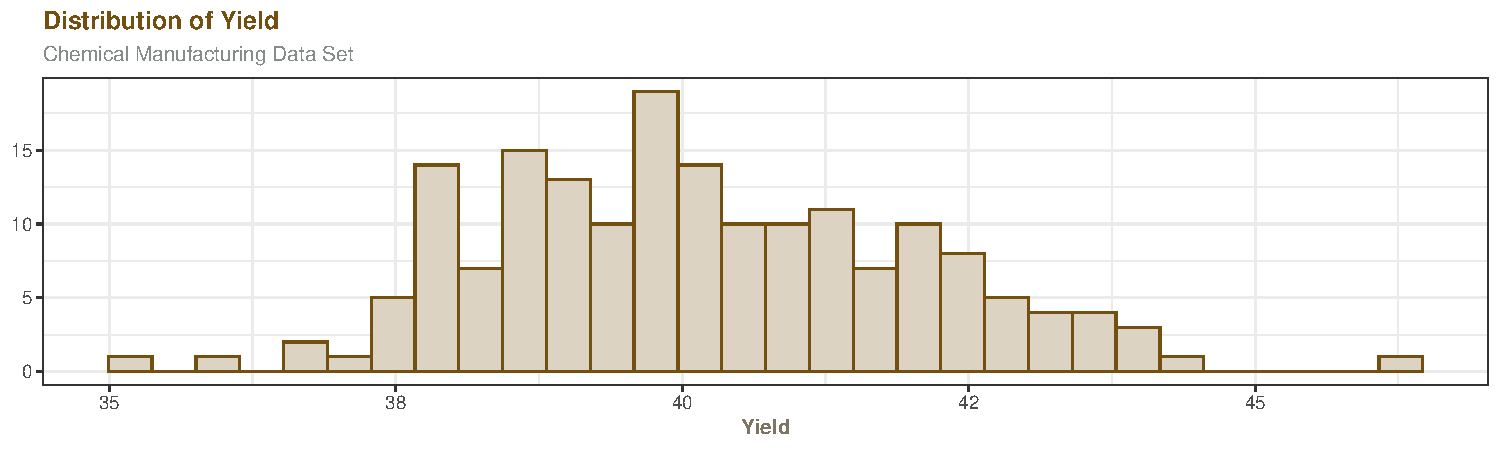
\includegraphics{Homework-Two_files/figure-latex/kj-6.3a-plot-1} \end{center}

\begin{subquestion}{(b).} A small percentage of cells in the predictor set contain missing values. Use an imputation function to fill in these missing values (e.g., see Sect. 3.8). 
\end{subquestion}

\texttt{ManufacturingProcess03} has the largest volume of missing data
followed by \texttt{ManufacturingProcess11}. Given that each variable
has less than 25\% of data missing, we should introduce methods of
imputation. For our purposes, we will use the MICE method. MICE is
formally known as Multiple Imputation with Chained Equations. On a high
level, MICE is built off a technique known as the Gibbs sampler.

The Gibbs sampler is a Markov chain based on Monte Carlo. MICE iterates
drawing estimates of missing values and parameters related to the
distribution of said variables. Chained equations are generally faster
than the Monte Carlo based Gibbs sampler. MICE has 5 imputations listed
as its default. Predictive mean matching is also a default method for
MICE. PMM does a better job at keeping non-linear relationships within
individual variables.

In addition to MICE, we drop variables that have near zero variance,
however we point out that only one variable was dropped. We still
include it as a process step to follow the literature's specifications.
After completing MICE, we no longer had missing data in our set. We
examined other imputation methods such as KNN but determined that there
was no significant change in the summary statistics across different
imputation methods.

\begin{table}[H]

\caption{\label{tab:kj-6.3b}Variables with Missing Values}
\centering
\fontsize{8}{10}\selectfont
\begin{tabular}[t]{lr>{\bfseries\raggedright\arraybackslash}p{0.1cm}lr}
\toprule
\textbf{Predictor} & \textbf{n} & \textbf{ } & \textbf{Predictor} & \textbf{n}\\
\midrule
\rowcolor{gray!6}  ManufacturingProcess03 & 15 &  & ManufacturingProcess02 & 3\\
ManufacturingProcess11 & 10 &  & ManufacturingProcess06 & 2\\
\rowcolor{gray!6}  ManufacturingProcess10 & 9 &  & ManufacturingProcess01 & 1\\
ManufacturingProcess25 & 5 &  & ManufacturingProcess04 & 1\\
\rowcolor{gray!6}  ManufacturingProcess26 & 5 &  & ManufacturingProcess05 & 1\\
\addlinespace
ManufacturingProcess27 & 5 &  & ManufacturingProcess07 & 1\\
\rowcolor{gray!6}  ManufacturingProcess28 & 5 &  & ManufacturingProcess08 & 1\\
ManufacturingProcess29 & 5 &  & ManufacturingProcess12 & 1\\
\rowcolor{gray!6}  ManufacturingProcess30 & 5 &  & ManufacturingProcess14 & 1\\
ManufacturingProcess31 & 5 &  & ManufacturingProcess22 & 1\\
\addlinespace
\rowcolor{gray!6}  ManufacturingProcess33 & 5 &  & ManufacturingProcess23 & 1\\
ManufacturingProcess34 & 5 &  & ManufacturingProcess24 & 1\\
\rowcolor{gray!6}  ManufacturingProcess35 & 5 &  & ManufacturingProcess40 & 1\\
ManufacturingProcess36 & 5 &  & ManufacturingProcess41 & 1\\
\bottomrule
\end{tabular}
\end{table}

\begin{subquestion}{(c).} Split the data into a training and a test set, pre-process the data, and tune a model of your choice from this chapter. What is the optimal value of the performance metric? 
\end{subquestion}

We will build a PLS model also known as partial least squares. PLS is a
statistical method that fits a linear regression model by projecting the
feature variables and response variable to some new space via a mapping
function. Because of this projection mechanism, for both predictors and
the response, the method becomes bilinear or simply known as linear with
respect to each of the variable types. PLS also has certain advantages
over other methods such as being more robust to dealing with issues
arising from multicollinearity.

For our PLS model, we partitioned the data by taking 80\% of the data as
training and the remaining 20\% as testing subsets. We also apply center
and scaling arguments set to true. We built a standard PLS model and
evaluated the root mean summary areas to determine the optimal number of
components to select. We generate performance metrics for our best tune
below:

\begin{table}[H]

\caption{\label{tab:kj-6.3c}PLS Performance Metrics on Training Subset}
\centering
\fontsize{8}{10}\selectfont
\begin{tabular}[t]{rrr}
\toprule
\textbf{RMSE} & \textbf{Rsquared} & \textbf{MAE}\\
\midrule
\rowcolor{gray!6}  1.571 & 0.3735 & 1.1723\\
\bottomrule
\end{tabular}
\end{table}

Our Baseline PLS model generates a RMSE of 1.57. In addition, the model
captures 37.35 \% of data variability. We include the visualizations
pertaining to the train set cross-validation RMSE tunes and a plot
comparing the observed and predicted outcome from our model.

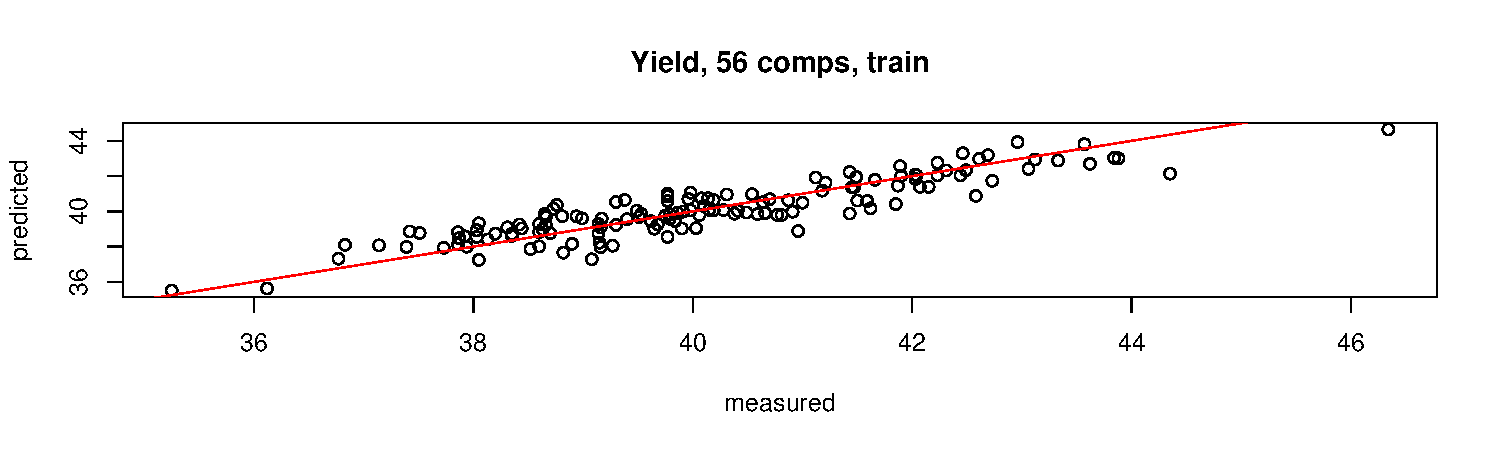
\includegraphics{Homework-Two_files/figure-latex/kj-6.3c2-1.pdf}

\begin{subquestion}{(d).} Predict the response for the test set. What is the value of the performance metric and how does this compare with the resampled performance metric on the training set? 
\end{subquestion}

We see a decreased R squared against the test data with 44\% of the data
variability accounted for. We also see the RMSE decrease to 1.55 from
our training results of 1.57. There is also a slight increase in the
MAE.

\begin{table}[H]

\caption{\label{tab:kj-6.3d-1}PLS Performance Metrics on Test Subset}
\centering
\fontsize{8}{10}\selectfont
\begin{tabular}[t]{rrr}
\toprule
\textbf{RMSE} & \textbf{Rsquared} & \textbf{MAE}\\
\midrule
\rowcolor{gray!6}  1.5506 & 0.4426 & 1.3058\\
\bottomrule
\end{tabular}
\end{table}

We also plotted the observed and predicted values from our test set
against each other below. The deviation from the fitted line tells us
that our selected linear model may not provide the best predictions for
\texttt{Yield}.

\begin{center}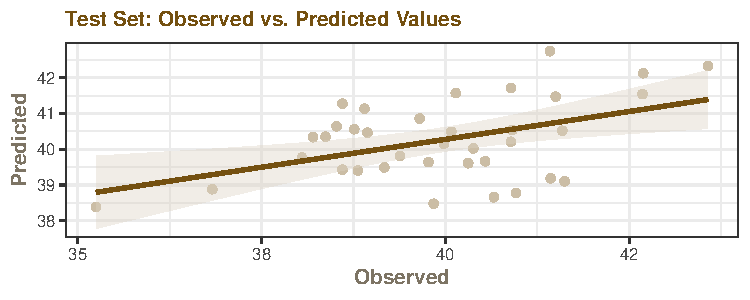
\includegraphics{Homework-Two_files/figure-latex/kj-6.3d-2-1} \end{center}

\begin{subquestion}{(e).} Which predictors are most important in the model you have trained? Do either the biological or process predictors dominate the list? 
\end{subquestion}

VarImp allows us to identify the variables by name and compute their
importance. \texttt{ManufacturingProcess32} was flagged as the most
important predictor overall and within the group of other Manufacturing
Process variables. \texttt{BiologicalMaterial06} ranked second and was
the most important variable within the BiologicalMaterial group. The
variable importance rankings are mixed with 7 variables belonging to
Biology and 8 Manufacturing Process variables within the top 15
predictors.

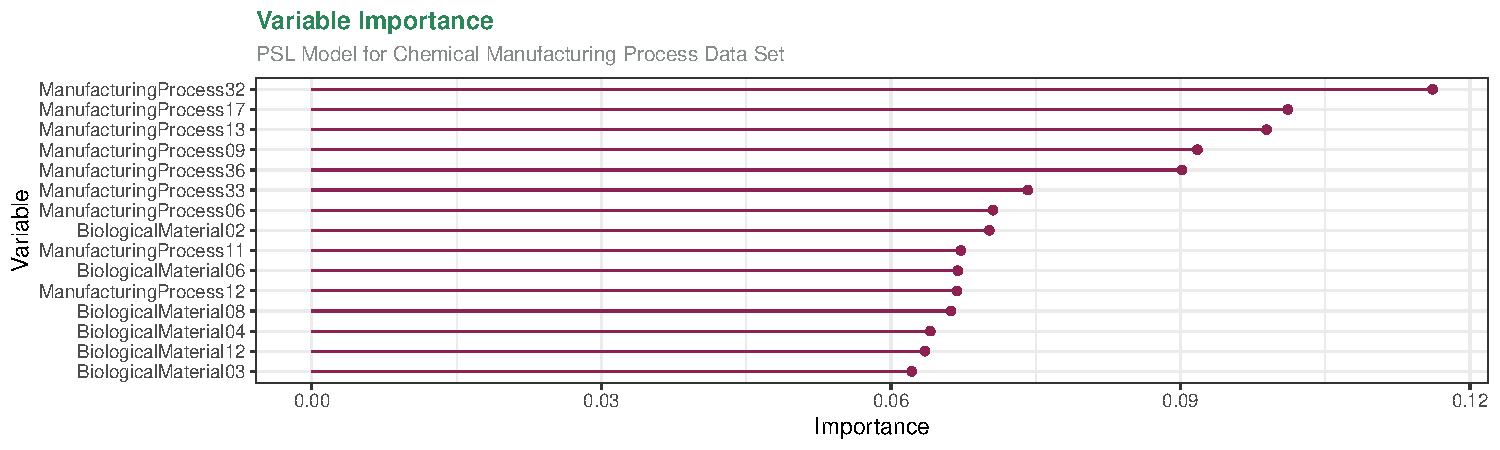
\includegraphics{Homework-Two_files/figure-latex/kj-6.3e-1.pdf}

\begin{subquestion}{(f).} Explore the relationships between each of the top predictors and the response. How could this information be helpful in improving yield in future runs of the manufacturing process?
\end{subquestion}

We used a scatter plot to visualize the relationship between our top
five important predictors against our response variable, \texttt{Yield}.
All but \texttt{ManufacturingProcess32} show a moderate positive, linear
relationship with yield.

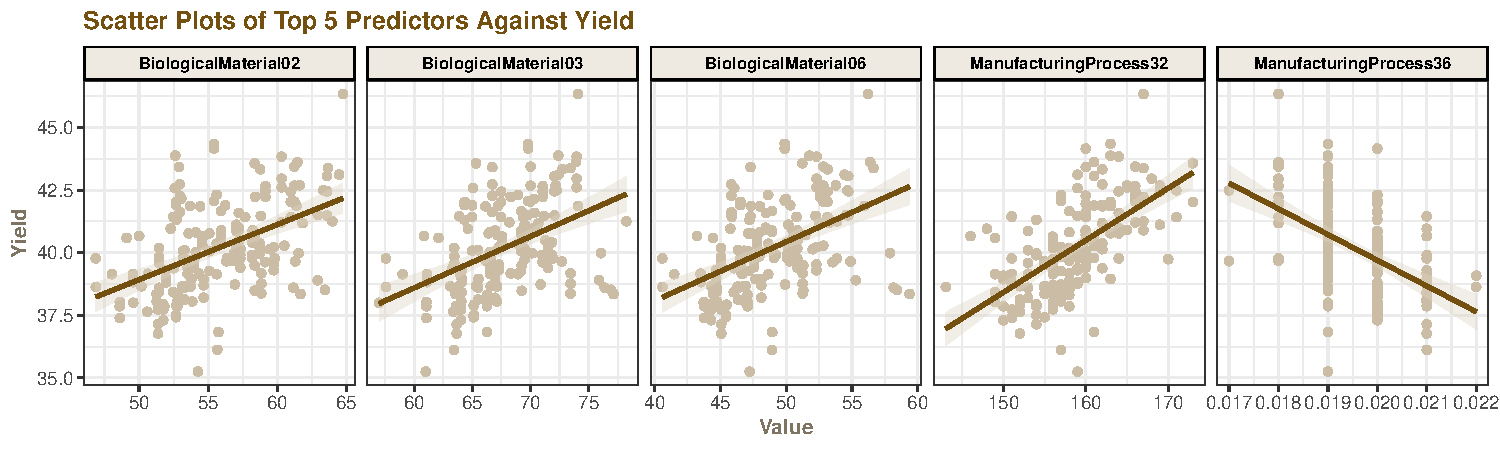
\includegraphics{Homework-Two_files/figure-latex/kj-6.3f-1-1.pdf}

We further examined this relationship by analyzing the correlation
strength between our top five important response variables with the
\texttt{Yield}. Out of which, \texttt{ManufacturingProcess32} showed the
strongest, positive correlation with our response variable.

From a business point of view, our aim is to increase yield since we
know that yield ties into revenue. We do not have insight into what
mechanics go into each manufacturing process but we can use this
knowledge to adjust the processes to emulate the highest yield outputs.

\begin{table}[H]

\caption{\label{tab:kj-6.3f-2}Variable Correlation with Yield}
\centering
\fontsize{8}{10}\selectfont
\begin{tabular}[t]{lr}
\toprule
\textbf{Variable} & \textbf{Yield}\\
\midrule
\rowcolor{gray!6}  ManufacturingProcess32 & 0.6083\\
ManufacturingProcess09 & 0.5035\\
\rowcolor{gray!6}  BiologicalMaterial02 & 0.4815\\
BiologicalMaterial06 & 0.4782\\
\rowcolor{gray!6}  ManufacturingProcess13 & -0.5037\\
\bottomrule
\end{tabular}
\end{table}

\hypertarget{AS-2}{%
\chapter*{Assignment 2}\label{AS-2}}
\addcontentsline{toc}{chapter}{Assignment 2}

\addcontentsline{toc}{subsection}{Kuhn and Johnson 7.2}

\begin{question}{Kuhn and Johnson 7.2}Friedman (1991) introduced several benchmark data sets create by simulation. One of these simulations used the following nonlinear equation to create data: $y = 10\text{sin}(\pi x_1 x_2)+20(x_3-0.5)^2+10x_4+5x_5+N(0\text{,} \sigma^2)$; where the $x$ values are random variables uniformly distributed between $[0, 1]$ (there are also 5 other non-informative variables also created in the simulation). 
\newline
The package `mlbench` contains a function called `mlbench.friedman1` that simulates these data. We convert the 'x' data from a matrix to a data frame. One reason is that this will give the columns names. The `testData` code creates a list with a vector 'y' and a matrix of predictors 'x'. It also simulates a large test set to estimate the true error rate with good precision: \end{question}

\begin{Shaded}
\begin{Highlighting}[]
\KeywordTok{set.seed}\NormalTok{(}\DecValTok{200}\NormalTok{)}
\NormalTok{trainingData <-}\StringTok{ }\KeywordTok{mlbench.friedman1}\NormalTok{(}\DecValTok{200}\NormalTok{, }\DataTypeTok{sd =} \DecValTok{1}\NormalTok{)}

\CommentTok{## We convert the 'x' data from a matrix to a data frame One}
\CommentTok{## reason is that this will give the columns names.}

\NormalTok{trainingData}\OperatorTok{$}\NormalTok{x <-}\StringTok{ }\KeywordTok{data.frame}\NormalTok{(trainingData}\OperatorTok{$}\NormalTok{x)}
\NormalTok{testData <-}\StringTok{ }\KeywordTok{mlbench.friedman1}\NormalTok{(}\DecValTok{5000}\NormalTok{, }\DataTypeTok{sd =} \DecValTok{1}\NormalTok{)}
\NormalTok{testData}\OperatorTok{$}\NormalTok{x <-}\StringTok{ }\KeywordTok{data.frame}\NormalTok{(testData}\OperatorTok{$}\NormalTok{x)}
\end{Highlighting}
\end{Shaded}

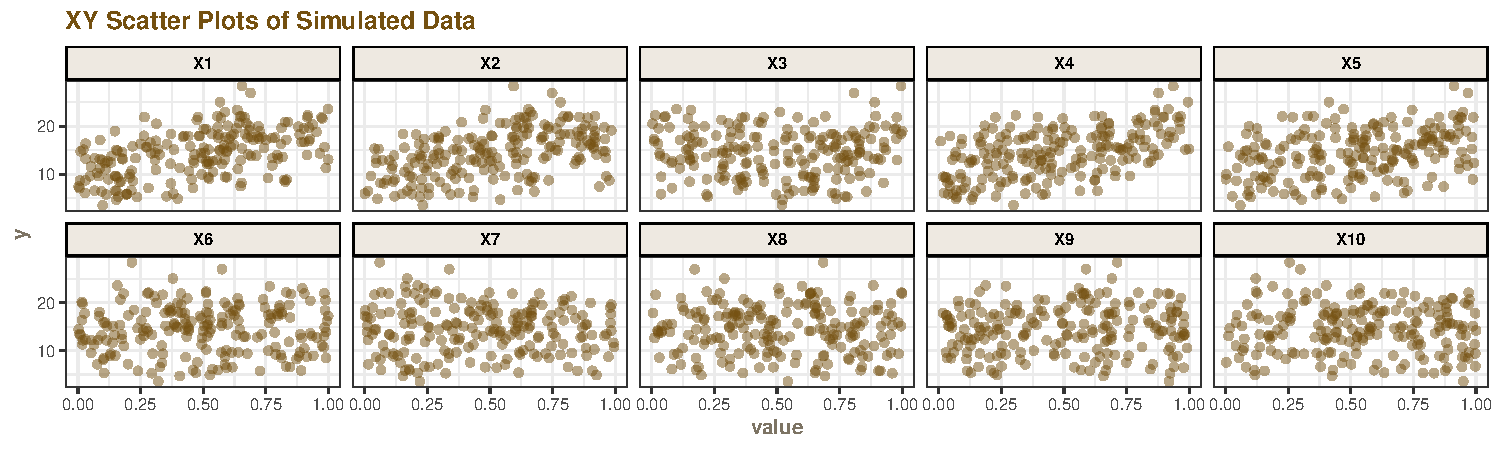
\includegraphics{Homework-Two_files/figure-latex/kj-7.2-ex3-1.pdf}

\begin{subquestion}{(a).} Tune several models on these data. For example: 
\end{subquestion}

\begin{Shaded}
\begin{Highlighting}[]
\NormalTok{knnModel <-}\StringTok{ }\KeywordTok{train}\NormalTok{(}\DataTypeTok{x =}\NormalTok{ trainingData}\OperatorTok{$}\NormalTok{x, }\DataTypeTok{y =}\NormalTok{ trainingData}\OperatorTok{$}\NormalTok{y, }\DataTypeTok{method =} \StringTok{"knn"}\NormalTok{, }
    \DataTypeTok{preProc =} \KeywordTok{c}\NormalTok{(}\StringTok{"center"}\NormalTok{, }\StringTok{"scale"}\NormalTok{), }\DataTypeTok{tuneLength =} \DecValTok{10}\NormalTok{)}
\NormalTok{knnModel}
\NormalTok{knnPred <-}\StringTok{ }\KeywordTok{predict}\NormalTok{(knnModel, }\DataTypeTok{newdata =}\NormalTok{ testData}\OperatorTok{$}\NormalTok{x)}
\KeywordTok{postResample}\NormalTok{(}\DataTypeTok{pred =}\NormalTok{ knnPred, }\DataTypeTok{obs =}\NormalTok{ testData}\OperatorTok{$}\NormalTok{y)}
\end{Highlighting}
\end{Shaded}

\#\#\#Model 1-MARS Regression:

MARS, otherwise known as multivariate adaptive regression splines is a
non-parametric regression technique that automatically captures
non-linearity and interaction between predictors. The basic MARS model
has the following form:

\[
\overset { \wedge  }{ f } =\sum _{ i=1 }^{ k }{ { c }_{ i }{ B }_{ i }(x) } 
\]

The model computes the sum of basis functions B multiplied by constant
coefficients C.The basis function can either be a constant, a hinge
function, or a product of hinge functions. By definition, a hinge
function is a piecewise function that converges at a point known as a
knot.

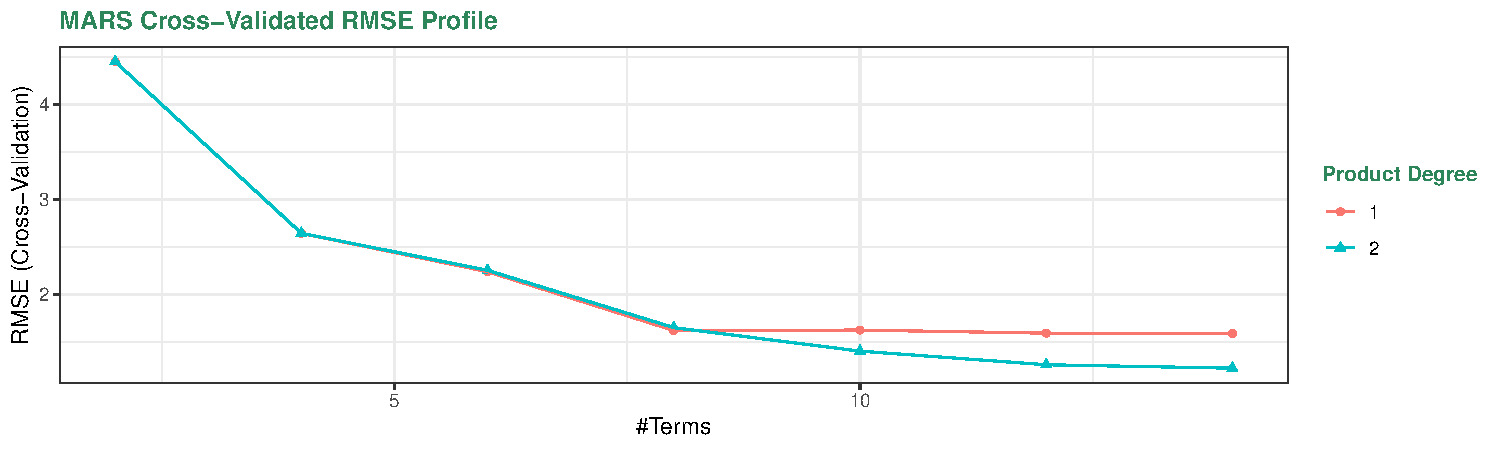
\includegraphics{Homework-Two_files/figure-latex/kj-7.2-1-1.pdf}

\#\#\#Model 2 SVM:

SVM, also known as support vector machine is a method that can be
applied to classification and regression tasks. On a high level, SVM
creates a hyperplane in n dimensional space. This hyperplane acts like a
classification boundary which can be linear or nonlinear. This boundary
classifies information from a feature space.

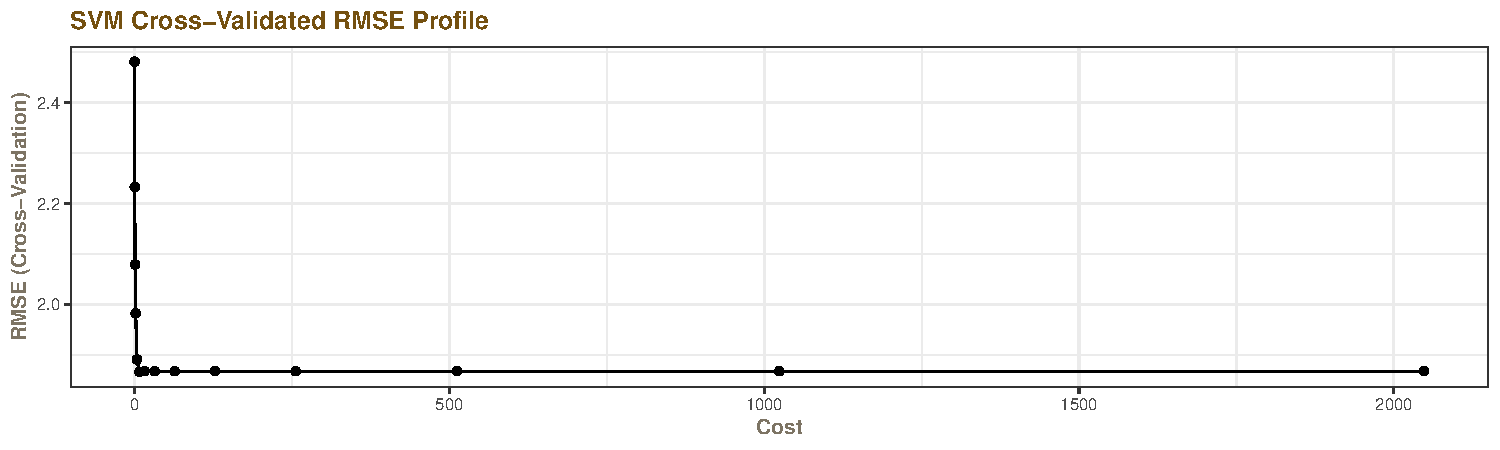
\includegraphics{Homework-Two_files/figure-latex/kj-7.2-2-1.pdf}

\#\#\#Model 3 NNET:

NNEt otherwise known as a Neural Network, is a method inspired by a
biological neuron system. It uses a system of nodes that are parallel to
the way neurons work. It is ideal for capturing non-linear relationships
that would otherwise be complicated in most multiple linear regression
models. NNET evolves internally based on the calculated weights of each
input. The basic structure is shown below:

\[
Y=\sum { (weight\quad *\quad input)\quad +\quad bias } 
\]

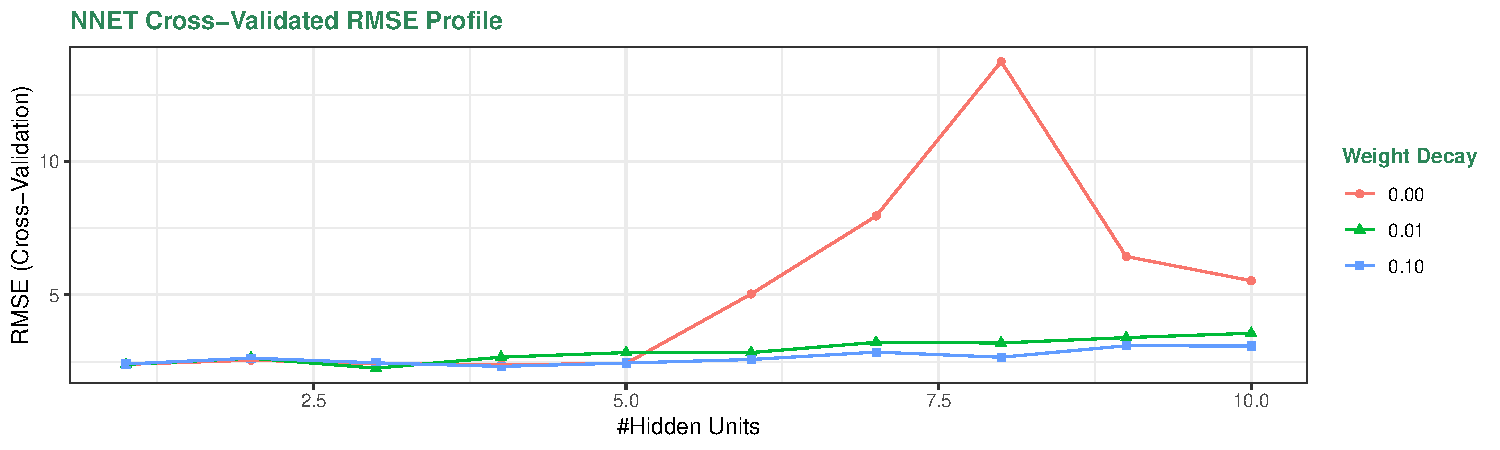
\includegraphics{Homework-Two_files/figure-latex/kj-7.2-3-1.pdf}

\begin{subquestion}{(b).}
Which models appear to give the best performance? Does MARS select the informative predictors (those named X1-X5)?
\end{subquestion}

\begin{table}[H]

\caption{\label{tab:unnamed-chunk-1}Model Performance}
\centering
\fontsize{8}{10}\selectfont
\begin{tabular}[t]{l|r|r|r}
\hline
\textbf{ } & \textbf{RMSE} & \textbf{RSquared} & \textbf{MAE}\\
\hline
\rowcolor{gray!6}  knnTrain & 3.6521 & 3.6521 & 3.6521\\
\hline
knnTest & 3.2041 & 0.6820 & 2.5683\\
\hline
\rowcolor{gray!6}  \rowcolor[HTML]{d9f2e6}  \textbf{MARSTrain} & \textbf{4.3290} & \textbf{0.9416} & \textbf{3.5906}\\
\hline
\rowcolor[HTML]{d9f2e6}  \textbf{MARSTest} & \textbf{1.1723} & \textbf{0.9449} & \textbf{0.9325}\\
\hline
\rowcolor{gray!6}  SVMTrain & 2.4814 & 0.8614 & 1.9813\\
\hline
SVMTest & 2.0425 & 0.8309 & 1.5491\\
\hline
\rowcolor{gray!6}  NNETTrain & 6.8166 & 0.7991 & 3.5714\\
\hline
NNETTest & 2.9888 & 0.6526 & 2.2931\\
\hline
\end{tabular}
\end{table}

MARS appears to give the best performance based on RMSE, R squared and
MAE on test set. The above table shows how our other selected models
stack up against the best performing MARS model. We now evaluate the
variable importance for our best performing model.

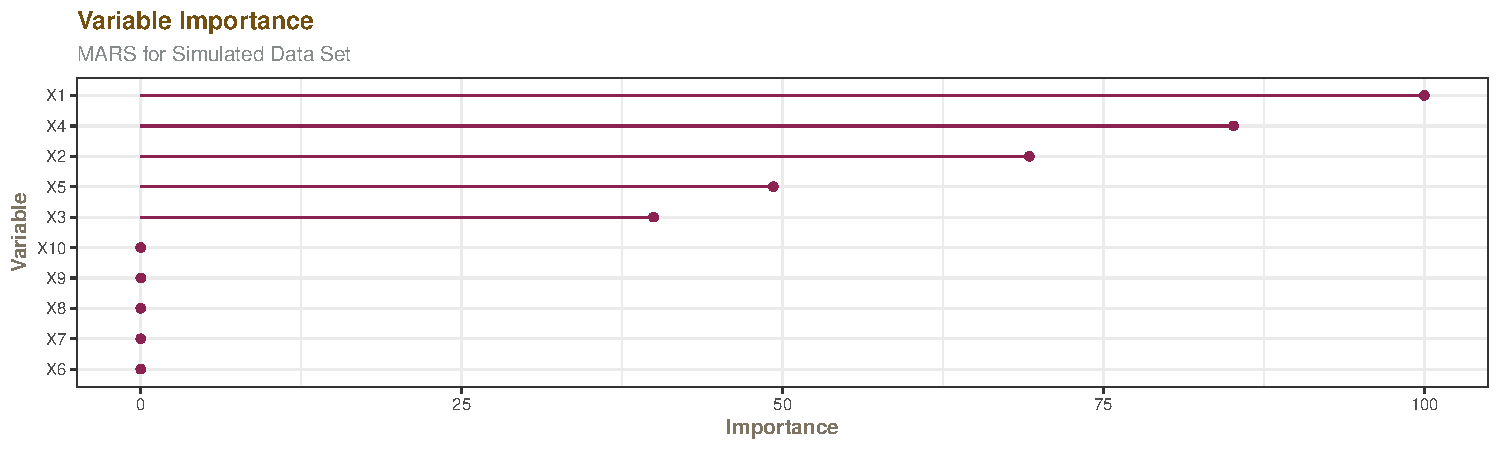
\includegraphics{Homework-Two_files/figure-latex/kj-7.2-4b-1.pdf}

The variable importance table for MARS indicates that variables X1
through X5 were picked as the most important. Out of our collection of
important variables used in MARS, X1 is the most important.

It is very likely that the lack of contribution allotted to the X6-X10
variables which bolster the R Squared and RMSE performance and noise
from these variables did not reduce the predictive strength of this
model as it does in small quantities in the other three models.

\addcontentsline{toc}{subsection}{Kuhn and Johnson 7.5}

\begin{question}{Kuhn and Johnson 7.5}
Exercise 6.3 describes data for a chemical manufacturing process. Use the same data imputation, data splitting, and pre-processing steps as before and train several nonlinear regression models.
\end{question}

We pulled in the data processing method from 6.3. This includes
imputation and removal of near zero variance features as processing
steps. Please refer to 6.3 for a more detailed look at the EDA involved
with this data set. We tuned a KNN model, NNET model, MARS, and SVM
model using specifications from the literature

\begin{subquestion}{(a).}
Which nonlinear regression model gives the optimal resampling and test set performance? 
\end{subquestion}

\begin{table}[H]

\caption{\label{tab:unnamed-chunk-1}Model Performance on ChemicalManufacturing Data}
\centering
\fontsize{8}{10}\selectfont
\begin{tabular}[t]{l|r|r|r}
\hline
\textbf{ } & \textbf{RMSE} & \textbf{RSquared} & \textbf{MAE}\\
\hline
\rowcolor{gray!6}  knnTrain & 1.4554 & 0.4344 & 1.1559\\
\hline
knnTest & 1.5151 & 0.4482 & 1.2684\\
\hline
\rowcolor{gray!6}  MARSTrain & 1.3809 & 0.6307 & 1.0786\\
\hline
MARSTest & 1.1999 & 0.6236 & 0.9192\\
\hline
\rowcolor{gray!6}  \rowcolor[HTML]{d9f2e6}  \textbf{SVMTrain} & \textbf{1.3678} & \textbf{0.6546} & \textbf{1.1134}\\
\hline
\rowcolor[HTML]{d9f2e6}  \textbf{SVMTest} & \textbf{1.2855} & \textbf{0.6030} & \textbf{0.9768}\\
\hline
\rowcolor{gray!6}  NNETTrain & 9.2718 & 0.3335 & 5.9237\\
\hline
NNETTest & 1.4996 & 0.4505 & 1.2194\\
\hline
\end{tabular}
\end{table}

Radial SVM outperformed the other models across all key KPIs. Radial SVM
is generally a more flexible basis function kernel than the base linear
kernel. The next best model was MARS regression. In part b, we will
address what variables are dominant in our SVM model.

\begin{subquestion}{(b).}
Which predictors are most important in the optimal nonlinear regression model? Do either the biological or process variables dominate the list? How do the top ten important predictors compare to the top ten predictors from the optimal linear model? 
\end{subquestion}

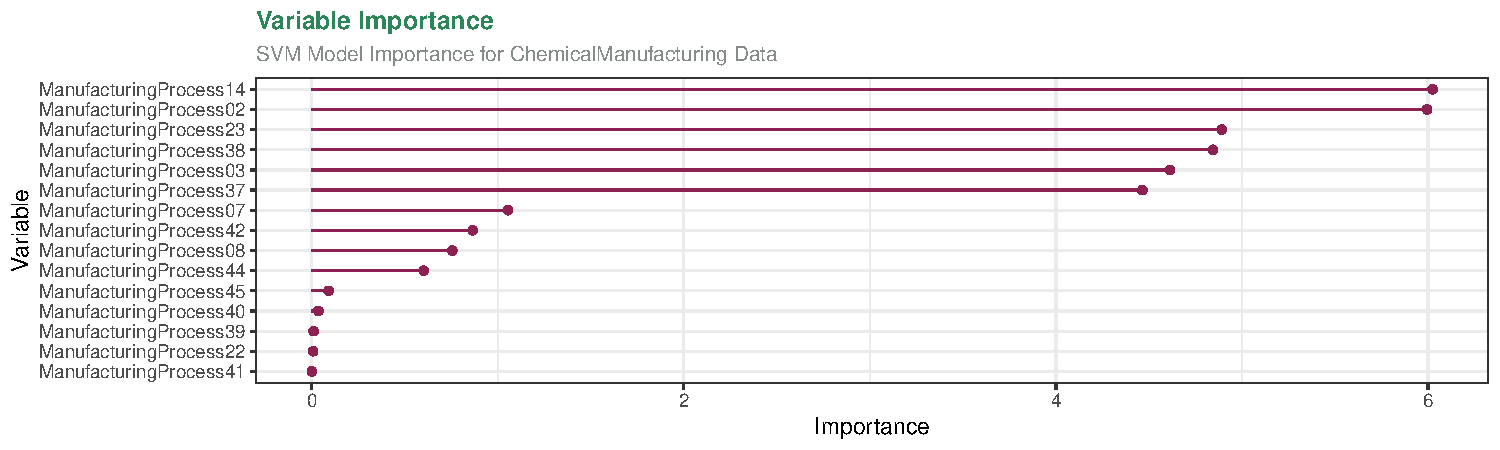
\includegraphics{Homework-Two_files/figure-latex/kj-7.5b-1.pdf}

\texttt{ManufacturingProcess} Variables dominate the ranking of
important variables with ManufacturingProcess14 at the top.
ManufacturingProcess32 was at the top of the important variables list
when it came to our linear model with some Biological Process within the
top 10.

\begin{subquestion}{(c).}
Explore the relationships between the top predictors and the response for the predictors that are unique to the optimal nonlinear regression model. Do these plots reveal intuition about the biological or process predictors and their relationship with yield?
\end{subquestion}

\begin{table}[H]

\caption{\label{tab:unnamed-chunk-1}Correlation}
\centering
\fontsize{8}{10}\selectfont
\begin{tabular}[t]{l|r}
\hline
VALUE & Yield\\
\hline
\rowcolor{gray!6}  Yield & 1.0000\\
\hline
ManufacturingProcess14 & -0.0100\\
\hline
\rowcolor{gray!6}  ManufacturingProcess38 & -0.0865\\
\hline
ManufacturingProcess03 & -0.1190\\
\hline
\rowcolor{gray!6}  ManufacturingProcess37 & -0.1593\\
\hline
ManufacturingProcess02 & -0.1954\\
\hline
\end{tabular}
\end{table}

We examined the top 5 predictors that were flagged as being the most
important before the importance measure dropped. There are some pretty
clear differences in the data which might explain both the overall poor
performance of the linear models as well as the improved significance of
Process-Based variables in the non-linear models.

Of the \texttt{ManfuacturingProcess} variables, they appear to be either
tight clusters or discrete values which predict an array of possible
Yields, which is directly opposed the definition of linearly separable
data base on earlier examination of correlation plots.

\hypertarget{AS-3}{%
\chapter*{Assignment 3}\label{AS-3}}
\addcontentsline{toc}{chapter}{Assignment 3}

\addcontentsline{toc}{subsection}{Kuhn and Johnson 8.1}

\begin{question}{Kuhn and Johnson 8.1} Recreate the simulated data from Exercise 7.2: \end{question}

\begin{subquestion}{(a).} Fit a random forest model to all of the predictors, then estimate the variable importance scores. Did the random forest model significantly use the uninformative predictors (V6-V10)?\end{subquestion}

The code to the RF model has been provided to us through the literature.

What is the code actually doing? We should dive into the theory. The
importance is calculated with the following formula:

\[
ni_j=W_{left(j)}C_{left(j)}-W_{right(j)}C_{right(j)}
\]

Let's deconstruct the theory. \(ni_j\) stands for node importance.
\(w_j\) is the weighted number of samples reaching node j. \(c_j\) is
the impurity value of node j. Left(j) is the child node from left split
on node j and right(j) is the child node from right split on node j.
Once \(ni_j\) is calculated, the importance for each variable on a
decision tree is calculated with formula I. Formula I is then normalized
as shown as formula II. The final feature importance is the average over
all trees. We simply find the sum of the features importance value and
then divide by all trees T, shown in formula III.

\[
I) \  fi_j \ =\frac{ (\sum_{j \ node \ split \ on \ i}) ni_j }{ ( \sum_{all \ nodes}) ni_k}\\
\]

\[
II) \  \parallel  fi_j  \parallel = \frac{(fi_j)}{\sum_{all \ features}fi_j} \\
\]

\[
III) \ RFfi_j= \frac{ ( \sum_{all \ trees})\parallel  fi_j \parallel}{T}
\]

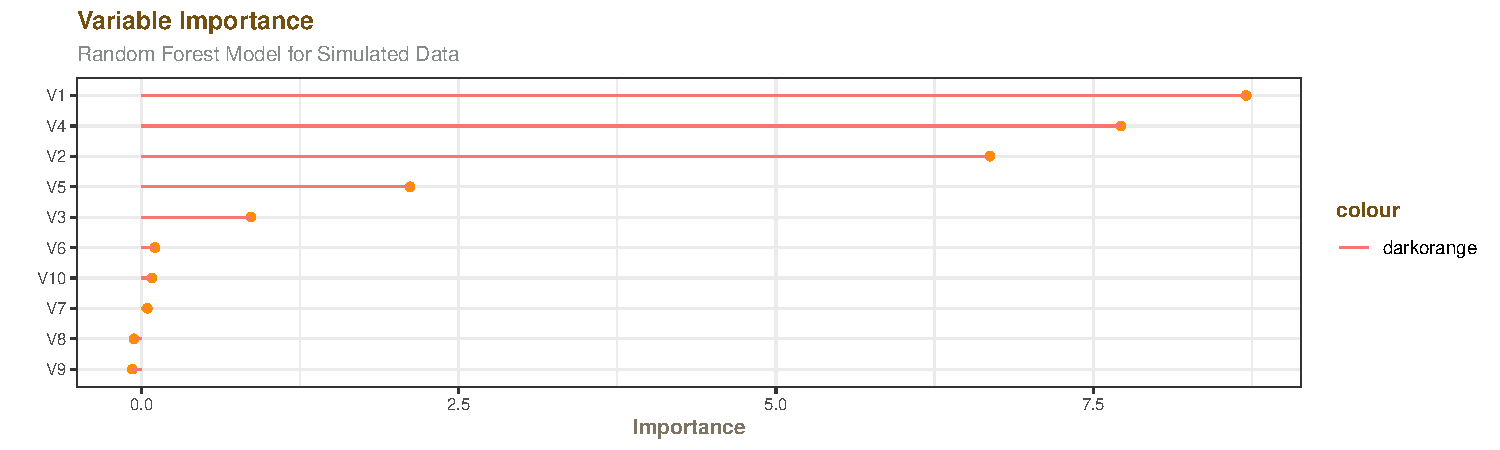
\includegraphics{Homework-Two_files/figure-latex/kj-8.1a-1.pdf}

Variables V6 to V10 were some of the least important variables, all with
a measure less than 1. Variables V1 through V5 were the most important
with variable V1 coming in at the top spot.

\begin{subquestion}{(b).} Now add an additional predictor that is highly correlated with one of the informative predictors. Fit another random forest model to these data. Did the importance score for V1 change? What happens when you add another predictor that is also highly correlated with V1? For example:\end{subquestion}

We add a feature that has a strong correlation of .93 with existing
feature V1. We will call this new feature \texttt{duplicate\ 1}

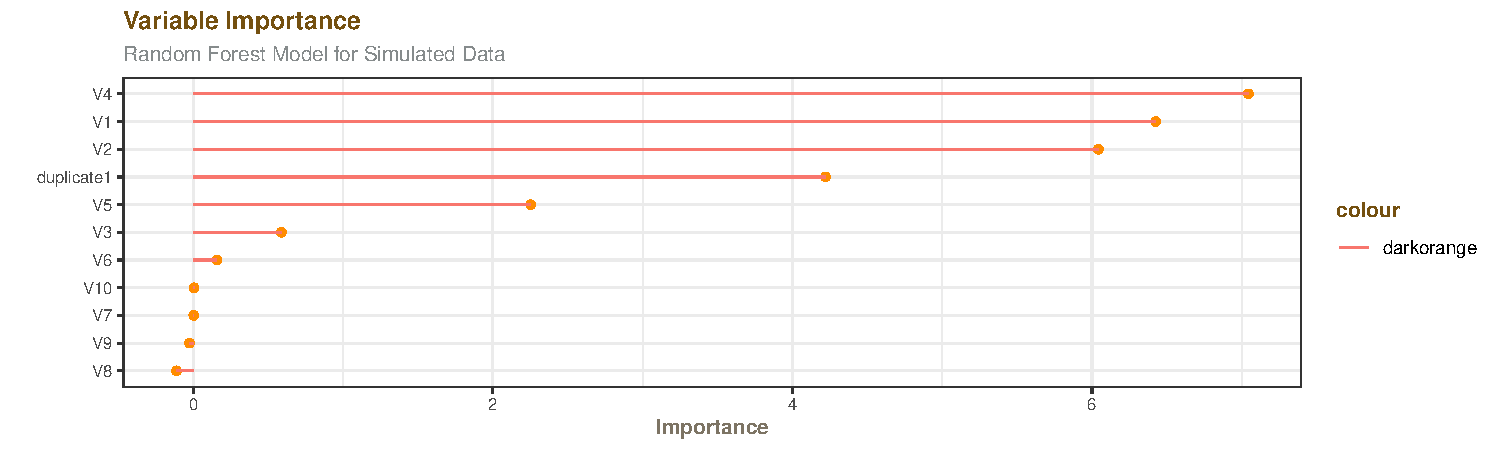
\includegraphics{Homework-Two_files/figure-latex/kj-8.1b-1.pdf}

Note that \texttt{V1} decreased importance by roughly 2 measures. V4 is
now the most important predictor. It looks like the importance score for
\texttt{V1} was partly absorbed by new predictor which underestimates
true importance of \texttt{V1} - the score sum of \texttt{V1} and
\texttt{duplicate1} are similar to the V1 score in (a). It makes sense
as \texttt{duplicate1} contains almost the same information as
\texttt{V1}.

\begin{subquestion}{(c).} Use the `cforest` function in the party package to fit a random forest model using conditional inference trees. The party package function `varimp` can calculate predictor importance. The `conditional` argument of that function toggles between the traditional importance measure and the modified version described in Strobl et al. (2007). Do these importances show the same pattern as the traditional random forest model?\end{subquestion}

\begin{table}[H]

\caption{\label{tab:unnamed-chunk-1}Conditional vs Unconditional CForest Model: Variable Importance}
\centering
\fontsize{8}{10}\selectfont
\begin{tabular}[t]{l|r|r|r|r|r|r}
\hline
\textbf{features} & \textbf{RF} & \textbf{CF} & \textbf{RF.cor} & \textbf{CF.cor} & \textbf{CF.cond} & \textbf{CF.cor.cond}\\
\hline
\rowcolor{gray!6}  duplicate1 & NA & NA & 4.2213 & 4.5798 & NA & 0.7636\\
\hline
V1 & 8.7065 & 10.0936 & 6.4252 & 4.9738 & 3.3655 & 0.7965\\
\hline
\rowcolor{gray!6}  V2 & 6.6871 & 7.5519 & 6.0433 & 7.2556 & 4.6869 & 4.2718\\
\hline
V3 & 0.8648 & 0.0516 & 0.5894 & 0.0020 & 0.0283 & 0.0062\\
\hline
\rowcolor{gray!6}  V4 & 7.7190 & 10.3981 & 7.0444 & 10.1938 & 5.8775 & 5.8944\\
\hline
V5 & 2.1172 & 2.2712 & 2.2531 & 2.2822 & 0.7146 & 0.8100\\
\hline
\rowcolor{gray!6}  V6 & 0.1072 & -0.0036 & 0.1589 & -0.0363 & 0.0099 & 0.0032\\
\hline
V7 & 0.0465 & 0.0576 & 0.0042 & 0.0276 & 0.0335 & 0.0006\\
\hline
\rowcolor{gray!6}  V8 & -0.0588 & -0.0496 & -0.1113 & -0.0431 & -0.0017 & -0.0062\\
\hline
V9 & -0.0717 & -0.0388 & -0.0242 & -0.0326 & -0.0043 & -0.0092\\
\hline
\rowcolor{gray!6}  V10 & 0.0822 & 0.0045 & 0.0062 & 0.0012 & 0.0112 & 0.0189\\
\hline
\end{tabular}
\end{table}

We performed both \texttt{varimp(,\ conditional\ =\ T)} and
\texttt{varimp(,\ conditional\ =\ F)} to compare \texttt{varimp} of
\texttt{cforest} in terms of permutation importance and conditional
permutation importance.

\begin{enumerate}
\def\labelenumi{\arabic{enumi}.}
\item
  RF vs CF Given that no correlated term is added, the importance
  pattern is similar except for the fact that V4 is now the most
  important feature in CF.
\item
  RF vs CF (with correlated term added) Given that correlated term is
  added, the importance score for \texttt{duplicate1} is much smaller in
  CF. This is the pin point difference between importance based on Gini
  coefficient (decision tree) and permutation test using p-value
  (conditional inference tree).
\item
  CF conditional vs CF with correlated term added and conditional When
  \texttt{conditional\ =\ T}, we perform conditional permutation test
  for measuring feature importance instead. Note that
  \texttt{duplicate1} has even smaller importance in
  \texttt{CF.cor.cond} than in \texttt{CF.cor}. For
  \texttt{CF.cor.cond}, notice \texttt{V1} became 3rd most important
  feature when it was 2nd most important for \texttt{CF.cor}. This is
  because conditional permutation helps uncovering the spurious
  correlation between \texttt{V1} and \texttt{duplicate1}.
\end{enumerate}

In summary, we learned that \texttt{CF} model surpresses the importance
score of \texttt{duplicate1} which helps maintain the importance of
\texttt{V1}. When \texttt{conditional\ =\ TRUE} in \texttt{varimp} for
\texttt{CF} model, the importance score of \texttt{duplicate1} is even
smaller.

\begin{subquestion}{(d).} Repeat this process with different tree models, such as boosted trees and Cubist. Does the same pattern occur?\end{subquestion}

Extracting the relative importance from a BGM object requires the use of
the native model summary.

\hypertarget{gbm-without-duplicate}{%
\subsubsection{GBM Without Duplicate}\label{gbm-without-duplicate}}

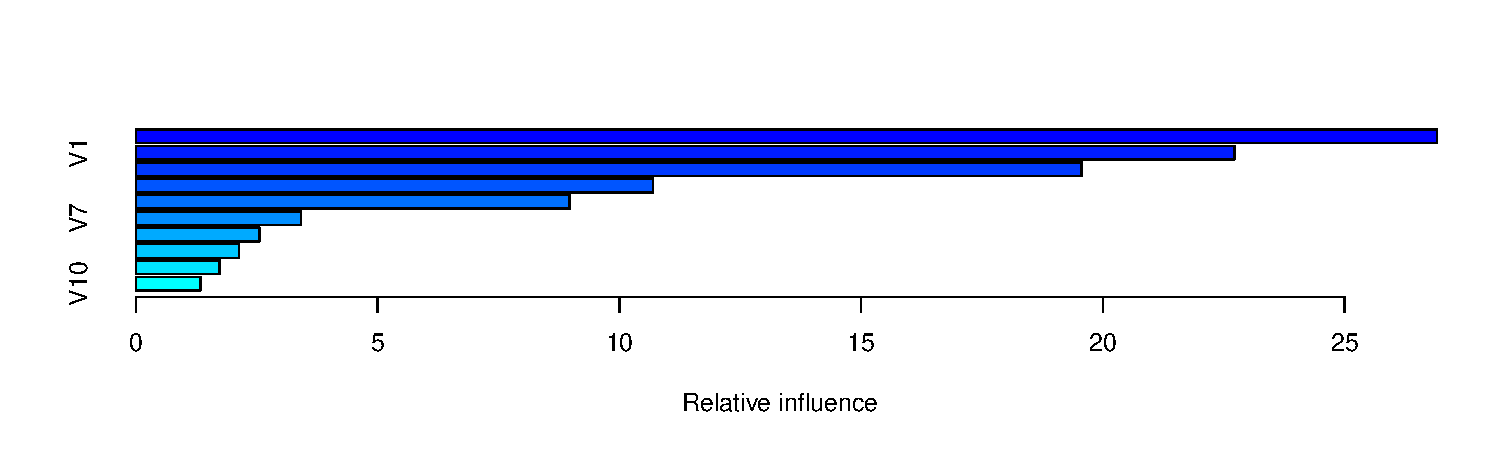
\includegraphics{Homework-Two_files/figure-latex/kj-8.1d-1.pdf}

\begin{verbatim}
    var   rel.inf
V4   V4 26.909998
V1   V1 22.717232
V2   V2 19.562270
V5   V5 10.691070
V3   V3  8.971001
V7   V7  3.408567
V6   V6  2.549782
V8   V8  2.130803
V9   V9  1.729656
V10 V10  1.329621
\end{verbatim}

\hypertarget{gbm-with-duplicate}{%
\subsubsection{GBM With Duplicate}\label{gbm-with-duplicate}}

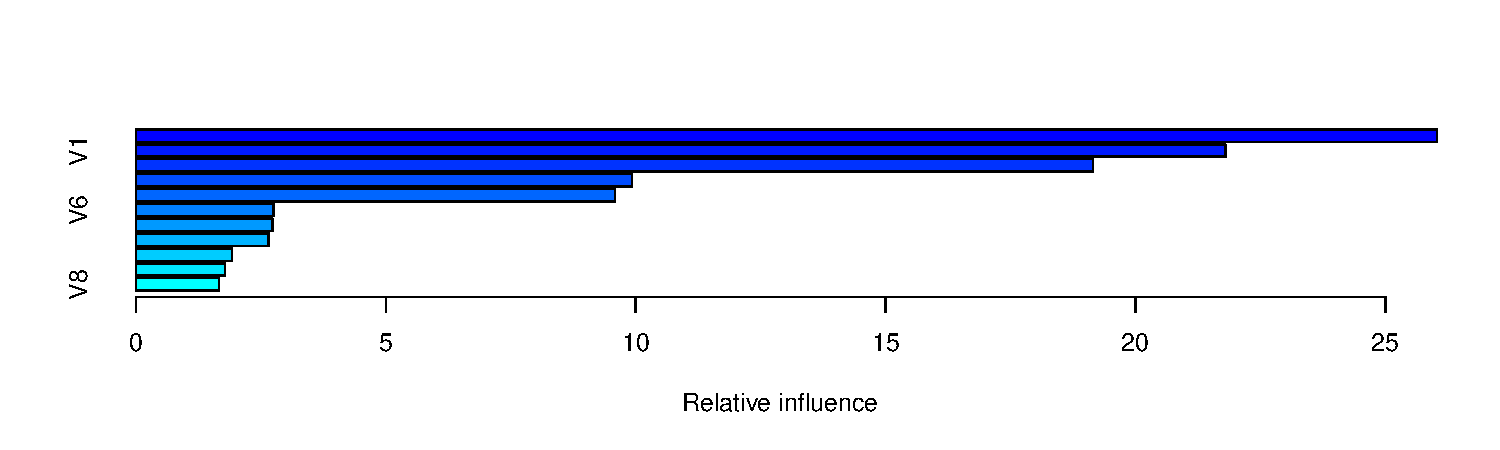
\includegraphics{Homework-Two_files/figure-latex/kj-8.1da-1.pdf}

\begin{verbatim}
                  var   rel.inf
V4                 V4 26.036164
V1                 V1 21.799842
V2                 V2 19.150149
V3                 V3  9.923707
V5                 V5  9.586174
V6                 V6  2.756297
duplicate1 duplicate1  2.729742
V7                 V7  2.656304
V10               V10  1.922812
V9                 V9  1.780691
V8                 V8  1.658119
\end{verbatim}

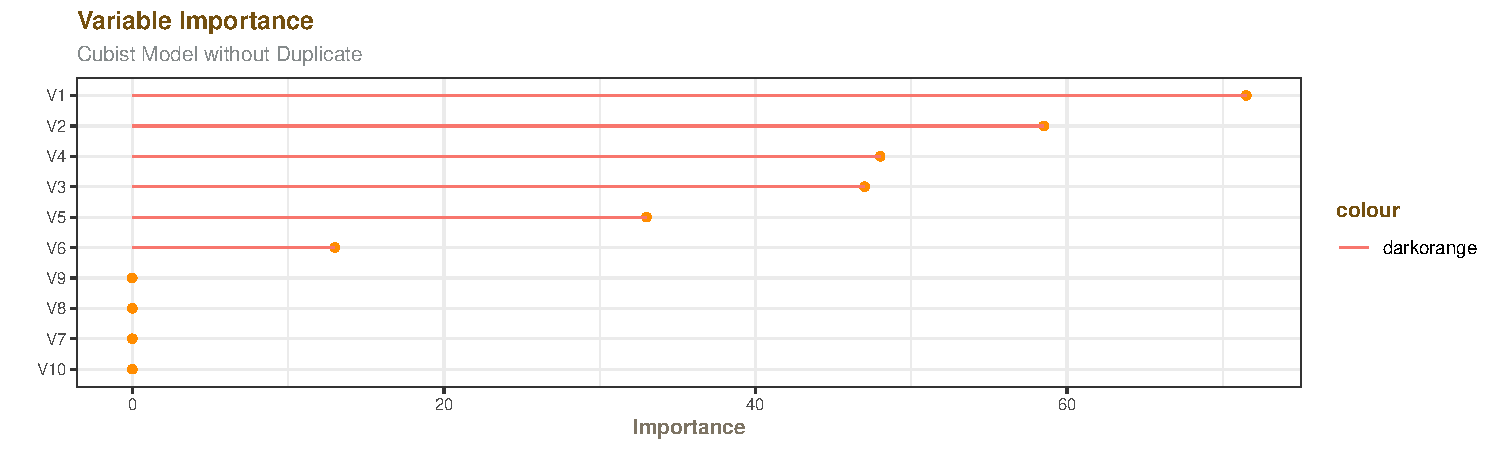
\includegraphics{Homework-Two_files/figure-latex/kj-8.1db-1.pdf}
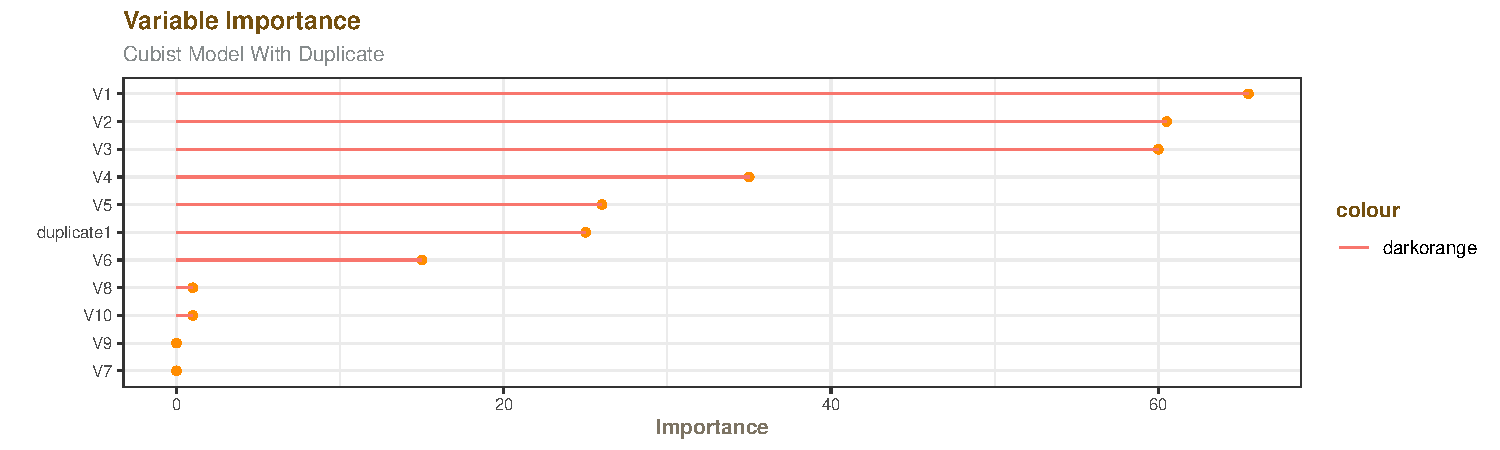
\includegraphics{Homework-Two_files/figure-latex/kj-8.1db-2.pdf}

The summary returns the variable name along with a measure of influence
on the target variable. From our GBM tree, we can see v4 is the most
influential. V1 and correlated duplicate1 are also much more
influential. V6-V10 does not break the top half of our list of
influential variables.

The next model we want to try is the cubist model. The cubist model is a
rather unique variation on trees. Each leaf in the tree contains a
linear regression model. Every layer in the tree alters the predicitons
used within each leaf contained model. In other words, the selection of
predictors in leaf n is based on the previous splis. It should be noted
that each intermediate step between leafs also contain a linear model.
Predictions are made via linear models on the on the terminal node.

\addcontentsline{toc}{subsection}{Kuhn and Johnson 8.2}

\begin{question}{Kuhn and Johnson 8.2}Use a simulation to show tree bias with different granularities.\end{question}

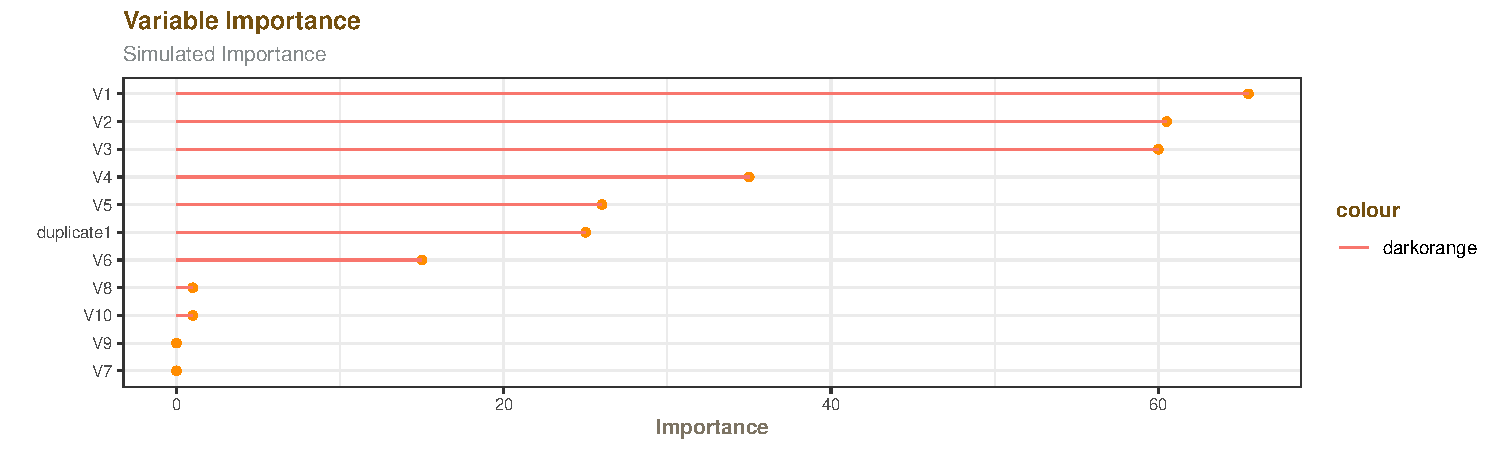
\includegraphics{Homework-Two_files/figure-latex/kj-8.2-1.pdf}

Basic regression trees split predictor variables into small groups based
on response variable. According to the literature, ``predictors with a
higher number of distinct values are favored over more granular
predictors.''

\addcontentsline{toc}{subsection}{Kuhn and Johnson 8.3}

\begin{question}{Kuhn and Johnson 8.3} In stochastic gradient boosting the bagging fraction and learning rate will govern the construction of the trees as they are guided by the gradient. Although the optimal values of these parameters should be obtained through the tuning process, it is helpful to understand how the magnitudes of these parameters affect magnitudes of variable importance. Figure 8.24 provides the variable importance plots for boosting using two extreme values for the bagging fraction (0.1 and 0.9) and the learning rate (0.1 and 0.9) for the solubility data. The left-hand plot has both parameters set to 0.1, and the right-hand plot has both set to 0.9: \end{question}

\begin{subquestion}{(a).} Why does the model on the right focus its importance on just the first few of predictors, whereas the model on the left spreads importance across more predictors? \end{subquestion}

Because the model on the right has hig learning rate and high bagging
fractions, it is doing two things, using 90\% of the variables in each
tree and using 90\% of the error for a given model. Imagine there were
ten variables in this model, if you used a bagging fraction of .9, the
every tree would have 9 of the ten trees in it, only one variable would
be different from the set of 9 trees in the first model each time. The
means that most of the possbile break-points in the trees would be the
same from tree to tree, only offering new opportunities for initial
splits when the most dominating variabl is removed. Because of this, you
would very likely find the model making the same first few decisions
each time. And with a learning rate of .9, 90\% of the error is added in
from each tree,this means that in addition to consistently choosing from
one or a few initial splits, you are also maximizing their contributions
to the models.

Because of these two factors, the trees contributing to the Stockastic
Boosted Tree in this example will make very few decisions (maening they
will make the same decisions repeately). That lack of variation in
initial choices means that the number of paths the learning can take is
limited, and with a high learning rate, a core set of variables is
selected early on from the trees built very similarly. In essence, the
model never has the opportunity to evaluate other possible variables
because the greediness of the model makes the same first few choices
every time(

\begin{subquestion}{(b).} Which model do you think would be more predictive of other samples?\end{subquestion}

The .9, .9 model would likely be overfit to the training data, because
the variation in values within those most important variables may not be
reflective of the general population. So, this model will be tuned to
choose from sample members following the samples distribution of values
in those most important features at the expense of recognizing
potiential splits in other variables which might be more common in the
poolation that the sample.

With a learning rate of .1 and a bagging fraction of .1, the left model
is more likely to build truly weak predictors, from smallers sets of
variables, consider more distinct breaking points, and therefore extend
better to wild data not fully described by the first few variables in
the importance summarise\_layers

\begin{subquestion}{(c).} How would increasing interaction depth affect the slope of predictor importance for either model in Fig.8.24?\end{subquestion}

Increasing the tree depth would affect both models, but differently. The
model with bagging fraction and learning rate equal to .1, increasing
the number of nodes in the tree would likely increase the importance of
the lower variables, creating a less polynomial slope. this is because
making more decisions, means giving weight the variables and values
where those decisions are made. This would give importance to those
variables.

For the model with bagging fraction and learning rate equal to .9,
increasing the depth would likely not change the slope of the lower
variables much at all just ad new variable or two to the top. The
difference is that in this model, with the high fraction and learning
rate, we again will still be making most of the same decisions, from
tree to tree, so the only increases in importance come from the added
nodes, which will be downstream, and they too are highly likely to be
the same from tree to tree, such that you will add a importance low on
the scale to those variables upon which the new nodes break (or upper
variables with a second or third break will grow in importance). So you
might see a reshuffling of upper nodes and the slight increase of a one
or two less important variables. However, the overall slope, of quickly
going to zero will be contrained by the high bagging fraction and
learning rate.

\addcontentsline{toc}{subsection}{Kuhn and Johnson 8.7}

\begin{question}{Kuhn and Johnson 8.7}
Refer to Exercises 6.3 and 7.5 which describe a chemical manufacturing process. Use the same data imputation, data splitting, and pre-processing steps as before and train several tree-based models:
\end{question}

\begin{subquestion}{(a).} Which tree-based regression model gives the optimal resampling and test set performance? \end{subquestion}

\begin{table}[H]

\caption{\label{tab:unnamed-chunk-1}Tree Model Performance on ChemicalManufacturing Data}
\centering
\fontsize{8}{10}\selectfont
\begin{tabular}[t]{l|r|r|r}
\hline
\textbf{ } & \textbf{RMSE} & \textbf{RSquared} & \textbf{MAE}\\
\hline
\rowcolor{gray!6}  GBM & 1.4978 & 0.6302 & 1.1941\\
\hline
GBMTest & 1.2073 & 0.6372 & 0.9550\\
\hline
\rowcolor{gray!6}  RFTrain & 1.2292 & 0.5546 & 0.9343\\
\hline
RFTest & 1.1859 & 0.6702 & 0.9286\\
\hline
\rowcolor{gray!6}  \rowcolor[HTML]{d9f2e6}  \textbf{CubistTrain} & \textbf{1.0567} & \textbf{0.7246} & \textbf{0.8118}\\
\hline
\rowcolor[HTML]{d9f2e6}  \textbf{CubistTest} & \textbf{1.0630} & \textbf{0.7183} & \textbf{0.8187}\\
\hline
\end{tabular}
\end{table}

The cubist model is the most optimal based on the r squared value.
Cubist both on the train and test data has a lower \texttt{RMSE} across
the different tree models we selected.

\begin{subquestion}{(b).} Which predictors are most important in the optimal tree-based regression model? Do either the biological or process variables dominate the list? How do the top 10 important predictors compare to the top 10 predictors from the optimal linear and nonlinear models?\end{subquestion}

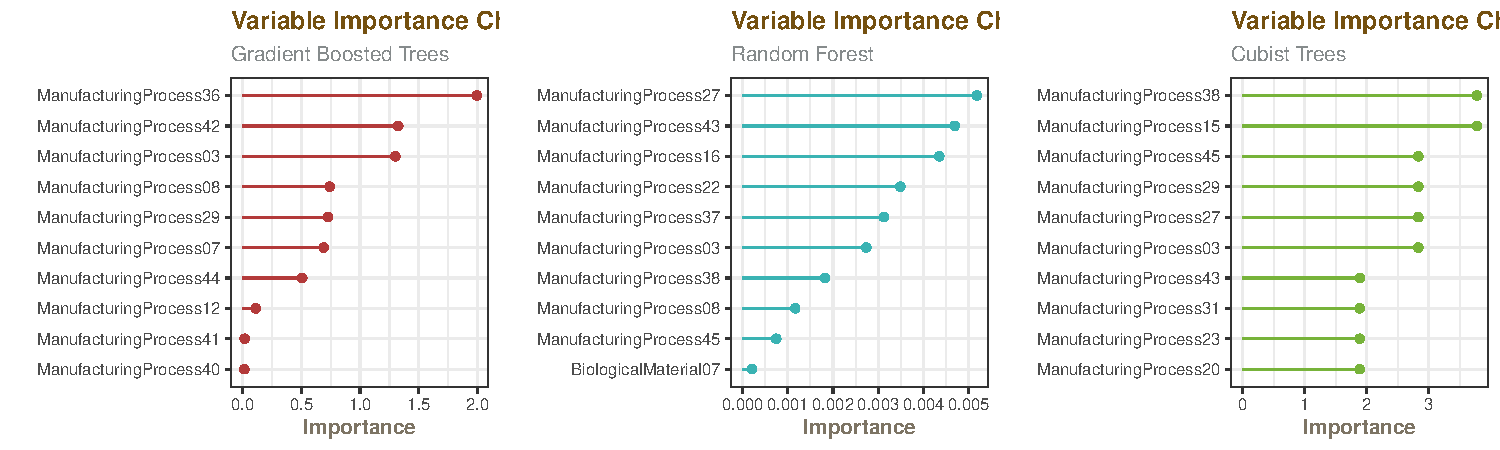
\includegraphics{Homework-Two_files/figure-latex/kj-8.7b-1.pdf}

In all the models the Manufacturing processes dominate the list, with
slight differences on where in the list and how much influence each has.

Comparing the top 10 variables in each model reveals some strong
differences. the Boosted tree follows a rather linear drop-off of
importance through a list of exclusively process-based variables. The
random forest falls off slower in the first five variables but becomes
rapidly linear. All but the last variable in this list are also process
based, the last is a biological material variable. The cubist tree,
however takes on a very different depreciation, as the values are
discrete, with the next six process variables all at exactly thre and
the last three variables at 2. Other than the first and last variables
all of the cubists top 10 are manufacturing process variable names.

\begin{subquestion}{(c).} Plot the optimal single tree with the distribution of yield in the terminal nodes. Does this view of the data provide additional knowledge about the biological or process predictors and their relationship with yield?\end{subquestion}

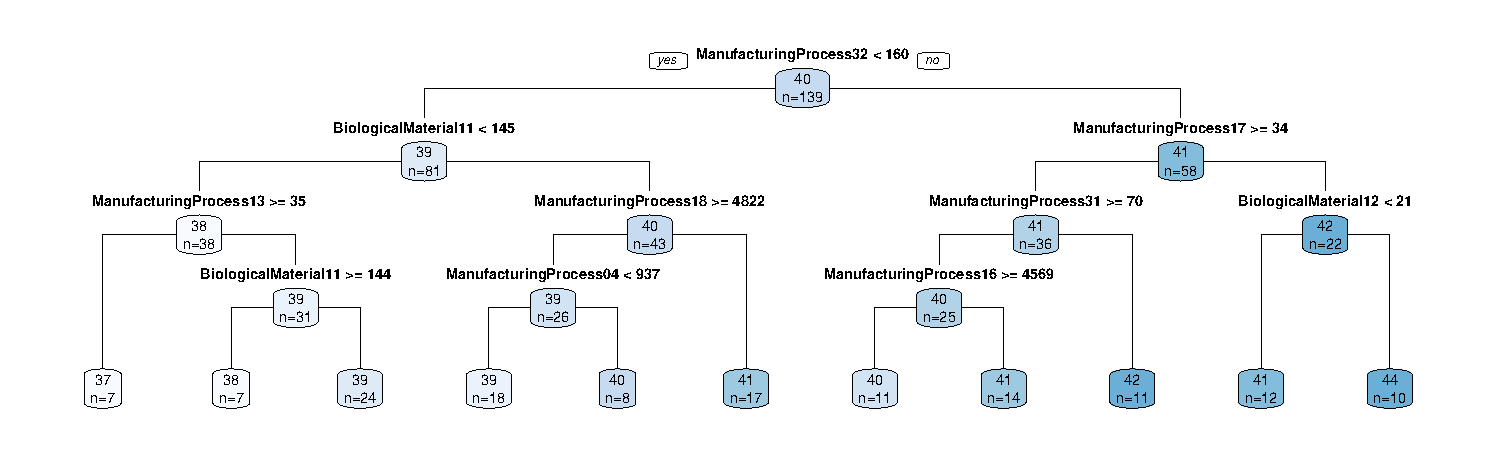
\includegraphics{Homework-Two_files/figure-latex/kj-8.7c-1.pdf}

Based on this regression tree, the differences between process and
matrial is that process variables differentiate more observations at
each break, which is why the break first, they increase the purity most
quickly. However, the final decisions seem to be based rather wholly on
biological material variables, such that only looking at Process or
prunning too soon, might lead to overfitting.

\hypertarget{AS-4}{%
\chapter*{Assignment 4}\label{AS-4}}
\addcontentsline{toc}{chapter}{Assignment 4}

\hypertarget{tbd}{%
\section{TBD}\label{tbd}}

\hypertarget{R-Script}{%
\chapter*{R Script}\label{R-Script}}
\addcontentsline{toc}{chapter}{R Script}


\end{document}
